%% LaTeX2e class for student theses
%% sections/evaluation.tex
%% 
%% Karlsruhe Institute of Technology
%% Institute for Program Structures and Data Organization
%% Chair for Software Design and Quality (SDQ)
%%
%% Dr.-Ing. Erik Burger
%% burger@kit.edu
%%
%% Version 1.3.3, 2018-04-17

\chapter{Evaluation}
\label{ch:Evaluation}
In diesem Schritt, soll die bisherige Arbeit evaluiert werden und dabei gezeigt werden, dass die definierten Ziele erreicht werden konnten. Diese sollen mithilfe der Goal-Question-Metric (GQM) definiert werden. Erste Überlegungen sind in \autoref{tab:gqm} definiert.\par
Das Vorgehen der Evaluierung ist in \autoref{abb:ablauf_evaluierung} abgebildet. Zunächst wird das Evaluierungssystem aufzusetzen. Dazu zählt sowohl die Implementierung, als auch eine Modellierung des Systems. Dieses Evaluierungssystem soll die Anforderungen erfüllen, die in \autoref{sec:systemanforderungen} definiert wurden. Nachdem das System eingerichtet wurde, soll eine Performanzanalyse der naiven Implementierung und der Modellierung des Systems stattfinden, damit ein Referenzwert gegeben ist. Pro Durchlauf soll, im Anschluss, sowohl eine MOM-Modellierung, als auch ihre Implementierung in das Evaluierungssystem eingesetzt werden. Anschließend wird eine Performanzanalyse der Systemimplementierung und der -Modellierung durchgeführt werden. Schließlich werden die Ergebnisse ausgewertet.

\section{Systemanforderungen}
\label{sec:systemanforderungen}
Für das Evaluierungssystem wurden im Folgenden Anforderungen festgelegt.
\begin{itemize}
\item Das jeweilige System soll \textbf{Skalierung} erlauben. Dabei soll es zum einen möglich sein die Anzahl von Kommunikationspartnern zu erhöhen (\textit{horizontal}) als auch die Menge an Nachrichten die verschickt werden (\textit{vertikal}).
\item Weitere \textbf{Konfigurationen} wie Nachrichtengröße, reihenfolgentreue, Duplikate, etc. sollten möglich sein.
\item System soll möglichst \textbf{reales System} darstellen.
\item Mindestens ein \textbf{Nachrichtenmodell} sollte unterstützt werden.
\item Es sollten \textbf{verschiedene Interaktionstypen} unterstützt werden, wie Many-To-Many, Many-To-One, etc.
\item Damit der Fokus der Masterarbeit auf den MOMs und ihrer Modellierung liegt, sollte das System \textbf{bereits vorhanden} und implementiert und modelliert sein.
\end{itemize}

\section{SPECJms2007}
Ein System das die in \autoref{sec:systemanforderungen} aufgestellten Anforderungen erfüllt ist das im SPECJms2007 Benchmark verwendete Testsystem \cite{Sachs2013}. Der Benchmark stellt eine reale ereignisbasierte Anwendung dar und umfasst eine Reihe von verschiedener Interaktionen, die sowohl Punkt-zu-Punkt- als auch Publish/Subscribe-Nachrichten einschließlich One-to-One-, One-to-Many- und Many-to-Many-Kommunikation umfasst. Das Hauptziel des SPECjms2007 Benchmarks ist es, einen Standard-Workload bereitzustellen, der die Leistung und Skalierbarkeit von JMS-basierten Message-Oriented Middleware-Plattformen bewertet. Bei dem System handelt es sich um ein Lieferkettenmanagement für eine Supermarktkette. Der Benchmark verwendet verschiedene Nachrichtentypen und verwendet Nachrichten verschiedenen Größe. Für die Masterarbeit liegt sowohl die Implementierung des Benchmarks, als auch eine Modellierung aus einer früheren Arbeit von Christoph Rathfelder \cite{Rathfelder2013} vor. Dieses System soll als Experimentsystem verwendet werden um die verschiedenen MOMs zu vergleichen und zum kalibrieren der später erstellten Modellierung. 

\subsection{Anwendungsszenario}
Das gewählte Anwendungsszenario bildet die Lieferkette eines Supermarktunternehmens ab. Beteiligte lassen sich wie folgt gruppieren: 
\begin{itemize}
    \item Hauptquartier (HQ): Für die Buchhaltung des Unternehmens verantwortlich. Beobachtet den Geld und Warenfluss im System. Verwaltet Informationen ueber Waren und definiert Preise.
    \item Supermarkt (SM): Verkauft Waren an Kunden. Im Benchmark liegt der Fokus auf der Verwaltung der eigenen Warenlager. Jeder SM ist mit einem Vertriebszentrum verbunden.
    \item Vertriebszentrum (DC): Beliefert SM mit Waren. Ein DC nimmt Aufträge von SMs an und liefert diese. Wenn ein DC die Waren nicht vorrätig hat, werden diese Waren von einem Zulieferer angefordert. Außerdem sind DCs dafür verantwortlich Verkaufsstatistiken an das HQ zu senden.
    \item Zulieferer (SP): SPs sind nicht Teil des Supermarktunternehmens. Jeder SP bietet eine bestimmte Art von Waren an. Diese werden an DCs geliefert, wenn angefordert.
\end{itemize}
In \autoref{img:specjmsInteraction} sind die vier Rollen zu sehen und wie sie miteinander kommunizieren. SpecJms sieht insgesamt sieben verschiedenen Interaktionsmöglichkeiten vor: 
\begin{itemize}
    \item Interaktion 1: Diese Interaktion modelliert die Auftrags- und Versandabwicklung zwischen SMs und DCs. Die Interaktion wird ausgelöst, wenn Waren im Lager eines SM aufgebraucht sind. Der SM bestellt bei einem DC Nachschub um seine Waren aufzufüllen. In \autoref{img:specjmsInteraction1} ist der Ablauf als Sequenzdiagramm abgebildet. Zunächst sendet der SM eine Order Nachricht an den DC. Der DC bestätigt dem SM den Eingang der Nachricht. Als nächstes werden die Waren verschickt. Dabei werden sie von einem RFID Leser erfasst. Schließlich sendet der DC Informationen über die Transaktion an das HQ. Sobald die Lieferung beim SM ankommt wird eine Bestätigung an DC gesendet.
\end{itemize}

\begin{figure}
\center
  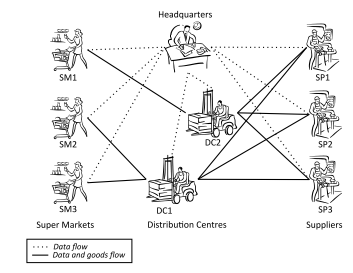
\includegraphics[width=1\textwidth]{images/specjms_scenario.png}
  \caption{Anwendungszenario des SpecJms}
  \label{img:specjmsInteraction}
\end{figure}
\begin{figure}
\center
  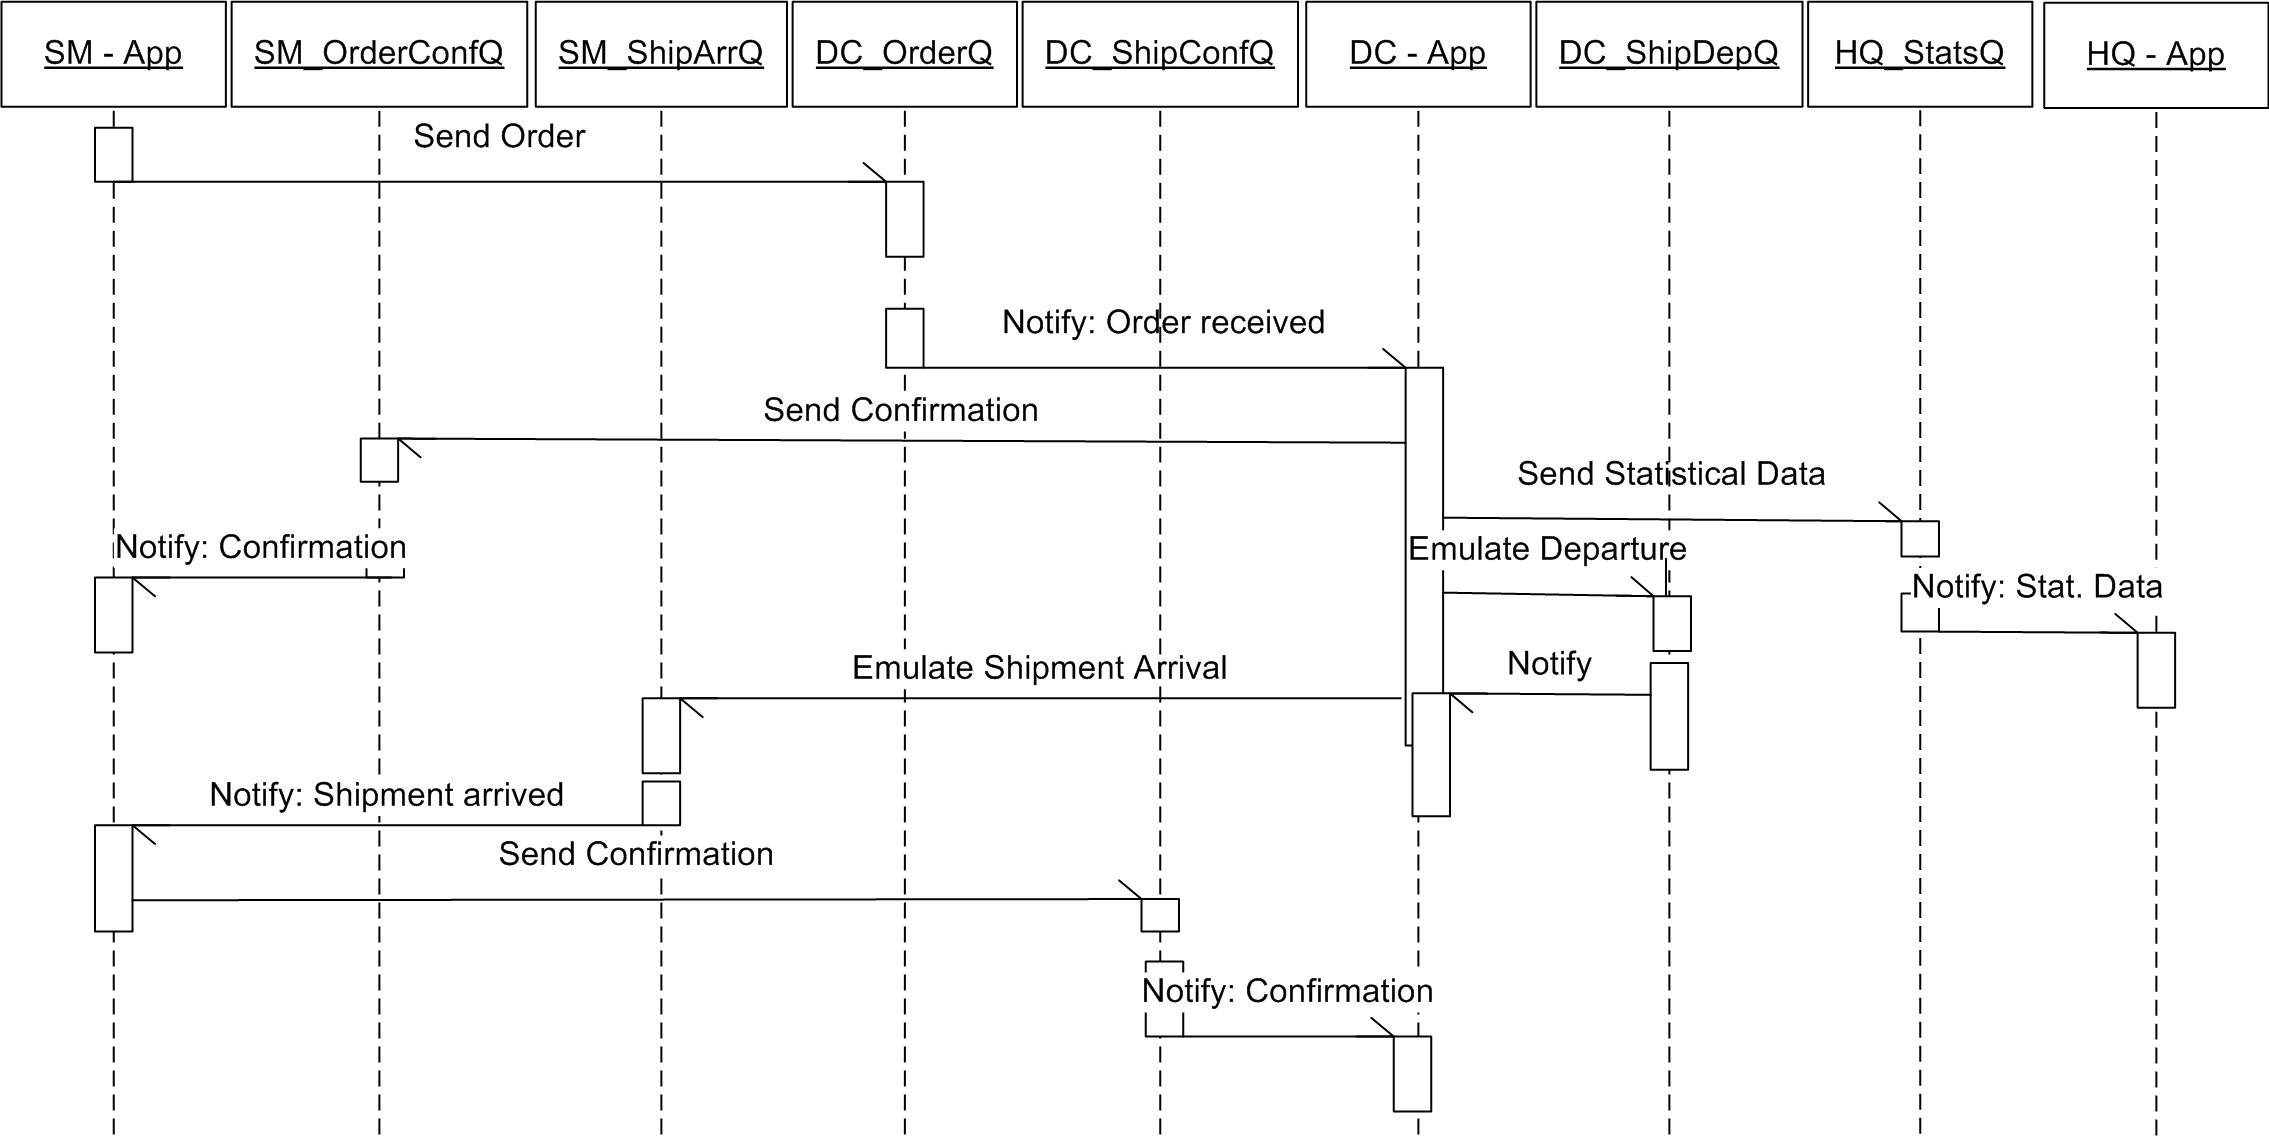
\includegraphics[width=1\textwidth]{images/Interaction1Diag.png}
  \caption{Interaktion 1}
  \label{img:specjmsInteraction1}
\end{figure}
Das System besteht aus vier Rollen, die in sieben verschiedenen Interaktionsmöglichkeiten miteinander kommunizieren können. 
Alle aufzaehlen\\
warum wurden nur 2 und wiese genau diese ausgewaehlt? (Zeit, welche kommunikationsarten konnten abgedeckt werden?)\\
Nachrichtenmodelle mit einbeziehen \\
Interaktionstypen mit einbeziehen \\
Szenario 1 (SM sendet Anfrage an DC)

Szenario 2 (DC muss Waren auffüllen)
%- 3 szenarios aus Dissertation \\
%- 1. alle interaktionen und p2p uns p/s \\
%- 2. teilmenge der interaktionen und fokus auf p2p \\
%- 3. teilmenge der interaktionen und fokus auf p/s \\

\subsection{Konfiguration}
Das System erlaubt verschiedene konfigurationen durch den Benutzer, wie die Skalierungsart oder die Nachrichtenröße. Das Szenario kann vertikal (Anzahl Msg (Produkte die verkauft werden) wird erhoeht, Consumer bleiben gleich) oder
hoizontal skalliert werden (Anzahl msg bleibt gleich, Consumer (SM) werden mehr)\\

Für jede Nachricht wird die Größe anhand festgelegter Parameter berechnet. Diese sind in \autoref{img:specjmsMsgSize} abgebildet. Die Größe wird mit folgender Formel berechnet: m1 + x * b, wobei x vom Benutzer des Benchmarks eingestellt werden kann.

\begin{figure}
\center
  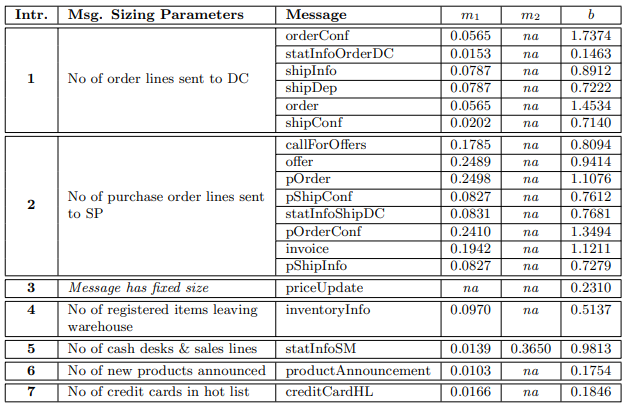
\includegraphics[width=1\textwidth]{images/specjmsmsgsize.png}
  \caption{Evtl. in Anhang}
  \label{img:specjmsMsgSize}
\end{figure}

\section{Beschreibung des Modells}
Modelle sind uebernommen worden aus diss. Nicht komplettes Modell beschreiben, sondern nur die Modelle der Interaktionen
\subsection{Repository}
\subsection{System}
Direkte Verbindung der Kommunikationen \\
RD innerhalb von Kommunikation (Verarbeitung von Nachrichten, bevor weiter geleitet, etc.)\\
Pub/sub ueber EventChannel \\
Start einer Interaktion wird durch Trigger ausgeloesst \\
\subsection{Ressource und Allocation}
\subsection{Usage}
\subsection{MOM}
RD fuer jede Moegliche Nachricht angegeben und davor ausgerechnet, siehe \autoref{img:specjmsMsgSizeRd} \\
\begin{figure}
\center
  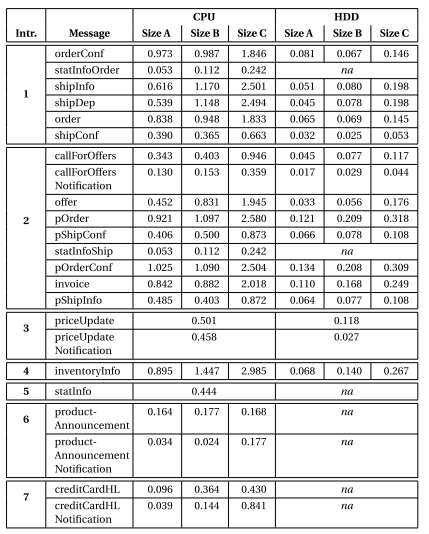
\includegraphics[width=1\textwidth]{images/specjmsmsgsizerd.png}
  \caption{Evtl. in Anhang}
  \label{img:specjmsMsgSizeRd}
\end{figure}


\subsection{Anpassung des Modells}
Meine Transformation wird verwendet anstatt Event Transformation \\
MOM Modell wird nicht verwendet\\
msg size wird nicht mehr in MOM fuer jede Nachricht berechnet und eingepflegt, sonder werden im UsageModell oder beim EmitEvent (incl) Verteilung mitgegeben \\

evtl ankunftsraten anpassen

\section{Goal-Question-Metric}
TODO aktualisieren \\
Die GQM-Methode \cite{gqm} spezifiziert Ziele für das zu validierende Konzept. Daraufhin werden zu den Zielen Fragen spezifiziert, mit denen die Erfüllung des Ziels überprüft werden soll. Schließlich werden Metriken festgelegt, durch die die Fragen beantwortet werden sollen. In \autoref{tab:gqm} sind erste Überlegungen festgehalten. Diese Überlegungen sind nicht vollständig und werden im Rahmen der Masterarbeit weiter ausgebaut.\par
Ein Ziel, das mithilfe dieser Masterarbeit erreicht werden soll, ist die Modellierung von MOMs in Palladio zu ermöglichen. Dafür wurden zwei Fragen definiert. Die erste Frage prüft ob sich MOMs überhaupt modellieren lassen. Die zweite Frage prüft die Modularität der MOM Bausteine. Das zweite Ziel ist, dass die Entscheidungsfindung, welche MOM verwendet werden soll, bereits zur Modellierungszeit und aus Architekturperspektive verbessert werden soll. Die dazu definierte Frage soll prüfen ob die Analyseergebnisse brauchbar, bzw. ob sich die Probleme einer Architekturentscheidung aus den Analyseergebnissen ableiten lassen. 
\begin{table}
  \begin{tabular}{|l|l|}
    \hline
    \multicolumn{2}{|l|}{Ziel 1} \\
    \hline
    Zweck & Ermögliche \\
    Qualitätskriterium & eine wartbare und wiederverwendbare Möglichkeit  \\ 
    Prozess & eine MOM zu modellieren \\
    Sicht & aus Architekturperspektive \\
   
    \hline \hline
    Frage 1 & Lassen sich MOMs modellieren? \\
    \hline
    Metrik & - Wie viele MOM Parameter konnten nicht modelliert werden? \\
    & - Wie viele Schritte müssen durchgeführt werden um eine neue \\
    & MOM zu modellieren\\
    \hline\hline
    Frage 2 & Wie modular sind die MOM Bausteine? \\
    \hline
    Metrik & - Wie viele Elemente müssen beim Austausch geändert werden? \\
    & - Min. Anzahl an Schritte um MOM auszutauschen \\
    \hline\hline
    \multicolumn{2}{|l|}{Ziel 2} \\
    \hline
    Zweck & Verbessere \\
    Qualitätskriterium & die Abwägung und Entscheidungsfindung  \\ 
    Prozess & beim Einsatz einer MOM \\
    Sicht & aus Architekturperspektive \\
    \hline \hline
    Frage 1 & Sind die Analyse Ergebnisse brauchbar? \\
    \hline
    Metrik & - Wie viel \% Abweichung zur naiven Modellierung/Implementierung? \\
    & - Wie viele Schritte müssen durchgeführt werden um Problem der \\
    & Architekturentscheidung aus dem Analyseergebnis abzuleiten? \\
    \hline
  \end{tabular}
	\caption{\label{tab:gqm} Ziele, Fragen und Metriken für die Evaluierung, nach der GQM-Methode}
\end{table}

\section{Modell vs Implementierung}
CPU Auslastung des Specjms vs. Modellierung\\
Response Time der einzelnen UsageScenarien aufaddieren um auf Interaction Time zu kommen. Vergleich mit Interaction time des Specjms\\
wie ist die Genauigkeit? Besser, gleich, schlechter\\


\section{Zusammenfassung}
Was ist das Ergebnis \\
Vergleich zu davor \\

%Modellierung eroeffnet neue moeglichkeiten\\

%\section{TIME}
%Ein weiteres System, das die Anforderungen aus \autoref{sec:systemanforderungen} erfüllt, ist das Transport Information Monitoring Environment (TIME) System \cite{time}. Dabei handelt es sich um ein System der Universität Cambridge. TIME soll ein reales Verkehrsüberwachungssystem darstellen. Es besteht aus mehreren verteilten Komponenten, die verschiedene Arten von Ereignissen senden bzw. empfangen. Die standardmäßige Middleware hat eine Peer-To-Peer Architektur, Punkt-zu-Punkt Kommunikation und unterstützt asynchronen Nachrichtenaustausch. Das System überwacht Autos mithilfe von Kennzeichenerkennung und soll den Verkehrsfluss optimieren. Diese Anwendung ist interessant, weil sie Daten von verschiedenen verteilten Sensoren und Systemen sammelt und integriert. Darüber hinaus enthält es Komponenten mit hohem und unterschiedlichem Ressourcenbedarf, wie z.B. der Kennzeichenerkennungsalgorithmus. Die Systemarchitektur ist sehr anpassungsfähig, wenn es darum geht, neue Komponenten hinzuzufügen oder die Verbindungen zwischen Komponenten oder deren Standort zu ändern. Was dazu führt, dass das hinzufügen und austauschen von verschiedenen MOMs möglich ist. Für die Masterarbeit liegt sowohl die Implementierung, als auch eine PCM-Modellierung des TIME Systems aus einer früheren Arbeit von Christoph Rathfelder \cite{Rathfelder2013} vor. Das TIME System soll für diese Masterarbeit als Evaluierungssystem dienen. Die Modellierung/Implementierung soll zunächst als Referenz für die Performanzanalyse dienen und im nächsten Schritt um verschiedene MOMs erweitert werden.